\documentclass[a4paper,
fontsize=11pt,
%headings=small,
oneside,
numbers=noperiodatend,
parskip=half-,
bibliography=totoc,
final
]{scrartcl}

\usepackage{synttree}
\usepackage{graphicx}
\setkeys{Gin}{width=.4\textwidth} %default pics size

\graphicspath{{./plots/}}
\usepackage[UKenglish]{babel}
\usepackage[T1]{fontenc}
%\usepackage{amsmath}
\usepackage[utf8x]{inputenc}
\usepackage [hyphens]{url}
\usepackage{booktabs} 
\usepackage[left=2.4cm,right=2.4cm,top=2.3cm,bottom=2cm,includeheadfoot]{geometry}
\usepackage{eurosym}
\usepackage{multirow}
%\usepackage[ngerman]{varioref}
\setcapindent{1em}
\renewcommand{\labelitemi}{--}
\usepackage{paralist}
\usepackage{pdfpages}
\usepackage{lscape}
\usepackage{float}
\usepackage{acronym}
\usepackage{eurosym}
\usepackage[babel]{csquotes}
\usepackage{longtable,lscape}
\usepackage{mathpazo}
\usepackage[normalem]{ulem} %emphasize weiterhin kursiv
\usepackage[flushmargin,ragged]{footmisc} % left align footnote
\usepackage{ccicons} 

%%%% fancy LIBREAS URL color 
\usepackage{xcolor}
\definecolor{libreas}{RGB}{112,0,0}

\usepackage{listings}

\urlstyle{same}  % don't use monospace font for urls

\usepackage[fleqn]{amsmath}

%adjust fontsize for part

\usepackage{sectsty}
\partfont{\large}

%Das BibTeX-Zeichen mit \BibTeX setzen:
\def\symbol#1{\char #1\relax}
\def\bsl{{\tt\symbol{'134}}}
\def\BibTeX{{\rm B\kern-.05em{\sc i\kern-.025em b}\kern-.08em
    T\kern-.1667em\lower.7ex\hbox{E}\kern-.125emX}}

\usepackage{fancyhdr}
\fancyhf{}
\pagestyle{fancyplain}
\fancyhead[R]{\thepage}

% make sure bookmarks are created eventough sections are not numbered!
% uncommend if sections are numbered (bookmarks created by default)
\makeatletter
\renewcommand\@seccntformat[1]{}
\makeatother


\usepackage{hyperxmp}
\usepackage[colorlinks, linkcolor=black,citecolor=black, urlcolor=libreas,
breaklinks= true,bookmarks=true,bookmarksopen=true]{hyperref}
%URLs hart brechen
\makeatletter 
\g@addto@macro\UrlBreaks{ 
  \do\a\do\b\do\c\do\d\do\e\do\f\do\g\do\h\do\i\do\j 
  \do\k\do\l\do\m\do\n\do\o\do\p\do\q\do\r\do\s\do\t 
  \do\u\do\v\do\w\do\x\do\y\do\z\do\&\do\1\do\2\do\3 
  \do\4\do\5\do\6\do\7\do\8\do\9\do\0} 
% \def\do@url@hyp{\do\-} 
\makeatother 

%meta
%meta

\fancyhead[L]{K. Bordonaro, S. Angalik \\ %author
LIBREAS. Library Ideas, 33 (2018). % journal, issue, volume.
\href{http://nbn-resolving.de/}
{}} % urn 
% recommended use
%\href{http://nbn-resolving.de/}{\color{black}{urn:nbn:de...}}
\fancyhead[R]{\thepage} %page number
\fancyfoot[L] {\ccLogo \ccAttribution\ \href{https://creativecommons.org/licenses/by/3.0/}{\color{black}Creative Commons BY 3.0}}  %licence
\fancyfoot[R] {ISSN: 1860-7950}

\title{\LARGE{Libraries and the Arctic: Language Education Support}} % title
\author{Karen Bordonaro, Shelby Angalik} % author

\setcounter{page}{1}

\hypersetup{%
      pdftitle={Libraries and the Arctic: Language Education Support},
      pdfauthor={Karen Bordonaro, Shelby Angalik},
      pdfcopyright={CC BY 3.0 Unported},
      pdfsubject={LIBREAS. Library Ideas, 33 (2018).},
      pdfkeywords={library, Arctic, language education, document analysis, Bibliothek, Arktis, Sprachausbildung, Dokumentenanalyse},
      pdflicenseurl={https://creativecommons.org/licenses/by/3.0/},
      pdfcontacturl={http://libreas.eu},
      baseurl={http://libreas.eu},
      pdflang={en},
      pdfmetalang={en}
     }



\date{}
\begin{document}

\maketitle
\thispagestyle{fancyplain} 

%abstracts
\begin{abstract}
The Arctic inspires awe. This unique region of the world has been
studied in many ways by many different disciplines. The discipline of
librarianship can also add to its study. In this article, the authors, a
practicing Canadian librarian at Brock University in Ontario and an
Inuktitut student enrolled at the same university, offer a suggested
role for libraries to play in the ongoing study of the Arctic. They
explore and describe the role of libraries in supporting native Arctic
language education. Support for learning and preserving native Arctic
languages can be found in library collections, spaces and services. This
article looks at support of native speakers and other interested
language learners, support of language research, support of language
preservation, and support of new publishing opportunities that can be
provided by or through libraries. These language support examples come
from a document analysis that perused web sites, conference proceedings,
published scholarship in the form of books and articles, newspaper
sources, and personal background knowledge of the authors. Documents
were collected, categorized, and described. The language support
categories that emerged illustrate the many different ways that
libraries can engage in native Arctic language education support. In
offering this role, the authors hope to provide a means for librarians
to learn more about the Arctic as well as a way for libraries to
contribute to knowledge of the Arctic.\\

Die Arktis weckt Ehrfurcht. Diese einzigartige Region der Welt wurde in
vielerlei Hinsicht von vielen verschiedenen Disziplinen untersucht. Die
Bibliotheksforschung kann auch dazu beitragen, die Arktis zu erkunden.
In diesem Artikel schlagen die Autorinnen, eine praktizierende
kanadische Bibliothekarin an der Brock University in Ontario und eine
Inuktitut-Studentin, die an derselben Universität eingeschrieben ist,
Bibliotheken eine Rolle in einer laufenden Studie zur Arktis vor. Sie
erforschen und beschreiben die Rolle von Bibliotheken bei der
Unterstützung der arktischen Sprachausbildung. Unterstützung bei dem
Erlernen und Bewahren der einheimischen arktischen Sprachen findet durch
die Bestände, Räumlichkeiten und Dienstleistungen der Bibliotheken
statt. Dieser Artikel befasst sich mit der Unterstützung von
Muttersprachlern und anderen interessierten Sprachstudenten sowie mit
der Unterstützung von Sprachforschung, Sprachbewahrung und von neuen
Veröffentlichungsmöglichkeiten, die von oder über Bibliotheken
bereitgestellt werden können. Die Beispiele für die Sprachunterstützung
stammen aus einer Dokumentenanalyse, die sowohl Websites,
Konferenzberichte, akademische Veröffentlichungen in Form von Büchern
und Artikeln und Zeitungsquellen als auch das persönliche
Hintergrundwissen der Autoren erforschte. Die Dokumente wurden
gesammelt, kategorisiert und beschrieben. Die auftretenden Kategorien
zur Sprachunterstützung illustrieren die mannigfaltige Art und Weise,
wie sich Bibliotheken an der Unterstützung der Sprache der Einheimischen
in der Arktis beteiligen können. Mit dieser Rolle hoffen die Autorinnen,
dass Bibliothekarinnen und Bibliothekare mehr über die Arktis erfahren
können und dass Bibliotheken einen Beitrag zum Wissen über die Arktis
leisten können.
\end{abstract}

%body
\hypertarget{introduction}{%
\section{Introduction}\label{introduction}}

The Arctic inspires awe. The sheer majesty of the landscape is often
imaged in visual form, as if words alone could not capture a full sense
of its essence. As a unique place on earth, its study can span many
disciplines -- science, history, ethnography, archaeology, and even
ecotourism, to name but a few. The discipline of librarianship does not
usually figure into its study or description.

This article seeks to serve as a small attempt to remedy the paucity of
knowledge about the Arctic in the general literature of librarianship.
It uses library support for Indigenous (more specifically Inuit) Arctic
language education as a way to open this door. This article describes
library programs, services, or collections that have the potential to
provide Indigenous Arctic language education support. The purpose of
this article is to consider the question: Is there a role for libraries
to play in Artic language education?

Language education support for Indigenous Arctic languages can take many
forms in and through libraries. The various forms that will be described
in this article include support for language use by Inuktitut and
Inuinnaqtun (or more generally Indigenous) speakers, language learning
purposes, language research purposes, language preservation, and new
publishing opportunities. Each will be described in this article and
illustrated through evidence of current practices taking place.

\hypertarget{personal-backgrounds}{%
\section{Personal Backgrounds}\label{personal-backgrounds}}

Brock University in southern Ontario, Canada, serves as the backdrop for
the writing of this article. One of the authors, Karen Bordonaro, is a
liaison librarian at the University who studies internationalization in
academic libraries, as well as linguistic uses of libraries by
non-Indigenous speakers of English in various settings within and
outside the United States and Canada. The other author, Shelby Angalik,
Inuk from Nunavut, is a current Brock undergraduate student majoring in
English who is considering the profession of librarianship as a possible
future career. Together, Karen and Shelby have gathered the information
that forms the main content of this article and have infused its
descriptions with their personal perspectives.

\hypertarget{arctic-connections}{%
\section{Arctic Connections}\label{arctic-connections}}

The personal language and library research interests of Karen and the
lived Inuk Arctic experiences of Shelby serve as the initial starting
background point for this article. Other starting points beyond our
personal settings, however, add further dimensions to our investigation
of Arctic language education support in and through libraries. These
further starting points encompass various connections between Brock
University and the Arctic, and between Canada and the Arctic that can
further add to the background of this article. In addition, connections
between Arctic language support and Canadian governmental policies, and
connections between Arctic language support and the literature of
librarianship can additionally broaden an understanding of the context
in which we are conducting our investigation. It should be noted at this
point, however, that the further starting points described below were
generally created by non-Indigenous people. So they do offer further
perspectives to consider, but they cannot be said to represent fully how
the Arctic can be understood or studied.

\hypertarget{brock-university-and-the-arctic}{%
\section{Brock University and the
Arctic}\label{brock-university-and-the-arctic}}

Brock University, though located at a sizeable geographic distance from
the Arctic in its base of operations in southern Ontario, nevertheless
has established some connections to the region. Shelby's physical
presence as a student at the University is the clearest example of a
connection between Brock and the Arctic.\footnote{\url{https://brocku.ca/brock-news/2016/07/nunavut-student-heading-to-brock-after-earning-td-scholarship-for-her-leadership-efforts/}}
Other examples exist as well, however, such as the Arctic solo travel
expedition engaged in by Adam Shoalts, an alumnus of the University as
described in both the alumni magazine (Firth, 2017) and online through
his own expedition web site.\footnote{\url{http://adamshoalts.com/expeditions/alone-across-arctic-2017/}}
And a final example of a Brock connection with the Arctic can be seen in
the hockey coaching work done by Joe Pelino, another Brock
alumnus.\footnote{\url{https://brocku.ca/brock-news/2017/08/brock-alum-raising-awareness-of-inuit-culture/}}

\hypertarget{canada-and-the-arctic}{%
\section{Canada and the Arctic}\label{canada-and-the-arctic}}

Canada, as a geographically located Northern country, has many obvious
connections with the Arctic. Many of these wider connections can be seen
in studies having to do with the climate or strategic location of the
Arctic and its importance for Canada as a nation (Griffiths, Huebert, \&
Lackenbauer, 2011; Zellen, 2013; Coad \& Reist, 2018). That the
government of Canada is supportive of these scientific investigations
concerning the Arctic is obvious as well (Campbell, 2017; Hoag, 2017).
And in addition to scientific and strategic investigations connecting
Canada with the Arctic, Canadian scholars also produce research that
considers historical, political, and artistic connections with the
Arctic (Zeller \& Ries, 2014; Charron, Plouffe, \& Roussel, 2012;
Rathwell \& Armitage, 2016). The exploration of larger sociological
concerns about how Indigenous Peoples (more specifically Inuit) in the
Arctic are represented and understood by non-Indigenous people in Canada
is also a subject of current study that connects Canada with the Arctic
(Johnston \& Tester, 2014). Perhaps at this juncture it would not be
remiss to note that the authors of this current article represent this
same duality, with Karen as a non-Indigenous and Shelby as an Inuk from
the Arctic.

\hypertarget{indigenous-languages-and-the-arctic}{%
\section{Indigenous Languages and the
Arctic}\label{indigenous-languages-and-the-arctic}}

In addition to connections between Brock University and the Arctic, and
the nation of Canada with the Arctic, there also exist connections
between language issues and government policies relating to the Arctic
that provide useful background information. Before considering such
issues, however, it may be useful at this juncture to offer some general
information about Indigenous Arctic languages here.

There is no one universal Indigenous Arctic language spoken by all
Indigenous people of the Arctic. In addition, the intersections of
Indigenous language, social culture and ethnic identity in this part of
the world add further nuances that are not easy for non-Indigenous
people to grasp (Dorais, pp.~293--308). In terms of language only, in
fact, the scope is enormous, and ever-changing. A review of a 1990 book
that came out under the auspices of the United Nations cultural arm,
UNESCO, for example, makes use of the term \enquote{Eskimo} that is no
longer considered acceptable terminology while also noting that,

\begin{quote}
\enquote{For the USSR, some 25 languages are covered in 107 pages; for
Alaska, Aleut and four varieties of Eskimo tone Inuit, three Yupik are
covered in 54 pages; for Canada, the Inuit dialect chain receives 105
pages; for Greenland (Greenlandic subsuming the local varieties of
Inuit) receives 74 pages; and for Northern Scandinavia, the varieties of
Sami (Lappish) are given 92 pages.} (Comrie, 1991, p.~625)
\end{quote}

Perhaps at this point, it would make sense to shift directly to Shelby's
voice alone in explaining what different kinds of Inuit languages can be
found in the Arctic:

There are many languages used by Inuit in Inuit Nunangat (Arctic regions
of Canada, Siberia, Alaska, and Greenland). But, in Canada, the two main
languages are Inuktitut (used in Nunavut and Nunavik) and Inuinnaqtun
(spoken in the Northwest Territories and Nunavut). There are many
similarities between languages spoken by Inuit, but there are also a lot
of differences. Dialects can differ from community to community and even
from family to family. More broadly, there is the Baffin dialect spoken
mostly in the northern parts of Nunavut, and the Kivalliq dialect spoken
mostly in the southern parts. For centuries, Inuktitut has been an oral
language, but with the introduction of settlers an Inuktitut alphabet
using syllabics was created in order to translate the Bible. The
syllabics from the Cree language were used and modified for Inuktitut.
Around the 1970's, the Makivik Corporation modified the written language
by removing the fourth column of the alphabet. Having now three columns
of the alphabet, it was much easier to use for printing and typing. Now,
the fourth column in only used in Nunavik.

Taking up the thread once again of connections, Arctic language
connections to government policies are also worth considering. Language
connections can be seen in examples such as the federal government of
Canada working with the province of Nunavut to \enquote{develop a
nationwide language law} (Pucci, 2017, p.~1) in order to protect
Indigenous languages of the Inuit, First Nations and Metis in
Canada.\footnote{{[}Footnote from the editorial team of LIBREAS. Library
  Ideas for non-canadian readers: Inuit are groups of indigenous
  peoples, living predominantly in the Canadian Arctic, Greenland and
  Alaska, First Nations is the umbrella term for other groups of
  indigenous people living in Canada. Métis are groups of people with
  mixed, indigenous and settler, ancestry.{]}} This is paralleled in
other parts of Canada as well, as in Nova Scotia where \enquote{the
chief of Nova Scotia's largest First Nation says he wants to pursue
talks with the provincial government about declaring Mi'kmaq an official
language in the province} (MacDonald, 2017, p.~1). The current language
concerns of Indigenous people are arising during a time of wider
reconciliation efforts across Canada to come to terms with corrosive
Indigenous legacies in the past (Gettler, 2017). This is a cultural
issue too complex to be easily summarized here, but it is well worth
noting as an important consideration in the broader backdrop to the
content of this article.

\hypertarget{libraries-and-the-arctic}{%
\section{Libraries and the Arctic}\label{libraries-and-the-arctic}}

Just as with language connections to the Arctic, so too can some
connections be found between libraries and the Arctic that can add
further helpful background information. Consulting the literature of
librarianship is a useful way to gain background information on how
librarianship may support or be practiced in the Arctic.

As implied at the start of the article, the literature of general
librarianship is not exactly rife with Arctic content. One exception
from the general literature, though, might be the library research done
on various aspects of internationalization within the realm of
libraries. This literature seeks to explore topics such as: notions of
intercultural understanding (Hall, 1992); widened understandings of
global literacy promotion (Global Literature in Libraries Initiative,
2017; Using Libraries to Support National Literacy Efforts, 2016); the
use of Indigenous versus non-Indigenous languages in libraries
(Gonzalez, 2017); the shared cataloguing, description, and community
input for Indigenous materials organization across libraries (Smith,
2008); and the importance of digitization projects involving Indigenous
language content (Sraku-Lartey, Acquah, Samar, \& Djagbletey, 2017). All
of these various aspects of general librarianship being studied could
potentially lend themselves to Arctic perspectives as well.

And all of above is not to say that absolutely no library work exists on
Arctic topics in the general literature of librarianship at all. There
is some literature available, often from Canadian library authors, which
will be referenced and used as examples in the next section of this
article. As a preview, it can be noted here that these Arctic library
articles found in this small subset of the literature touch on topics
such as delivery service, cataloguing, and providing materials in
Indigenous languages by practicing librarians in this region.

And in addition to these articles describing practices that will be
highlighted in the next section, some work on gathering Arctic research
material for librarians has taken place as well. For example, Spencer
Arcadia, an academic librarian in the United States, published a list of
Internet resources for the February 2011 issue of \emph{College \&
Research Libraries News} on \enquote{Arctic Research: Environment,
Health, and Culture of the Circumpolar North} (Arcadia, 2011). He is
also currently working on a forthcoming book tentatively titled
\enquote{\emph{Arctic Social Sciences and Humanities: The Role of
Library, Archival, and Information Sciences in the Circumpolar North}},
which could also widen the knowledge base for librarians.\footnote{\url{https://www.apecs.is/news/polar-news/1718-call-for-paper-proposals-arctic-social-sciences-humanities-and-the-roles-of-library-archival-and-information-sciences.html}}

Besides considering the library literature, a further useful way to
learn about libraries and the Arctic can be to consider its practice in
everyday library settings in this region. One very direct way to do this
is to consult local Arctic library associations operating in this region
of the world. An example of an association like this is the Nunavut
Library Association. Perusing their web site can give interested
librarians an inside look at how libraries operate in this very unique
setting, and what some of the opportunities and the challenges could be
in serving Inuit populations in Nunavut.\footnote{\url{https://nunavutlibraryassociation.ca}}

All of the connections and settings described above serve as contextual
background information for the main content of this article. This
information is meant to illuminate where the question of how libraries
can support Arctic language education came from. And it offers
interested librarians a brief glimpse at how Arctic library work can
potentially be understood and investigated.

\hypertarget{document-analysis}{%
\section{Document Analysis}\label{document-analysis}}

The main content of this article comprises examples of library practices
that illustrate the various ways that libraries can play a role in
supporting Indigenous language education in the Arctic. The evidence for
these various ways comes from identifying and collecting documents that
show or describe current library practices that either already support
or have the future potential to support Indigenous Arctic language
education in and through libraries.

The examples described below come from an array of different documents
that included web sites, conference notifications and proceedings, and
books and relevant articles from the literature of librarianship and
news sources that contain mentions of the Arctic. Documents were found
through general web searches, library databases such as LISTA (Library,
Information Science and Technology Abstracts), education databases such
as Education Source and ERIC, the new database iPortal (the Indigenous
studies portal research tool developed by the University of
Saskatchewan), book catalogues of Brock University Library and WorldCat,
regional newspaper and online radio sources, and from word-of-mouth and
the personal background knowledge of the authors.

The methodology used to analyze the documents followed a sequence of
collection, categorization, and description. Collected examples were
grouped by categories. The categories that emerged from this grouping
included library support of Indigenous Arctic language education through
these various ways: through language use, language learning, language
research, language preservation, and publishing opportunities. The
examples were then perused for content and details that could
potentially shed further light on a particular category. Examples were
aligned, and the following descriptions of practices below were
developed.

\hypertarget{language-support-examples}{%
\section{Language Support Examples}\label{language-support-examples}}

Libraries, whether public, school, or academic, can engage in Arctic
language education support in a multitude of ways. The ways below
illustrate a number of different options for other libraries that may
also be interested in playing a role in providing this support.

Once again, this seems to be an important place to hear Shelby's voice
directly. By describing her personal goals concerning the support of
literacy in the Arctic potentially through librarianship, she can offer
the rest of us a unique perspective on why Indigenous (or more
specifically Inuktitut or Inuit) Arctic language support could be an
important role for libraries to play.

Due to Inuit having more recently been colonized, we are still
transitioning and trying to find a happy middle in keeping our culture
alive but also keeping up with the times. Our language is a major part
of who we are. We have perspectives and thoughts that cannot be
translated into English, our culture is embedded within the language. I
am really interested in studying literacy in the western culture because
I gain new perspectives from reading in English as well. Growing up in a
generation stuck between two cultures, with one (western culture) being
forced more predominantly than the other (Inuit culture) has been
difficult but opened my eyes and probably others in my generation. With
literacy, I feel I can take from my Inuit culture and western literacy
and help Inuit youth in bettering their education, not necessarily only
in schools, but in everyday life as well. I cannot stress the importance
of Inuktitut enough. Having Inuktitut in our youth's day to day lives
will strengthen Inuit culture. As Inuit, what we need more is the help
from other Inuit when it comes to literacy, we need our own librarians
who can incorporate Inuit culture in every aspect of learning. I became
interested in literacy for children, especially Inuit youth. I want
Inuit youth to have the proper education that they need without
completely assimilating to the western culture, but instead
incorporating Inuit culture into the western culture. I was taught that
most Inuit are illiterate, by seeing all the statistics you would assume
so too. But that is only in the English language that many Inuit are
considered illiterate, not in Inuktitut. We have to understand that we
are an oral culture, for centuries our knowledge and values have been
passed down through storytelling. We are still transitioning into using
the written language. In the near future I would really like to see our
education system favour Inuit in every aspect of literacy, and blend
Inuktitut literacy and English literacy together.

Taking Shelby's words into account, the content of this article will now
shift to the categorized descriptions of examples collected from the
document analysis.

\hypertarget{language-use}{%
\section{Language Use}\label{language-use}}

For people who are already Indigenous speakers of Arctic languages,
libraries can most certainly support their further Indigenous language
use. This can be done through the incorporation of the Indigenous
language itself as a way to search the library's collections. For
example, the Nunavut Arctic College Library offers a \enquote{change
language} option on their web site for Indigenous speakers of
Inuinnaqtun and Inuktitut (see Figure 1 below).\footnote{\url{http://www.arcticcollege.ca/en/arctic-college-library-services}}

\begin{figure}
\centering
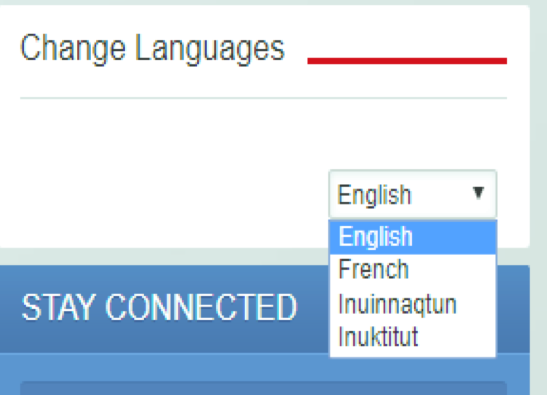
\includegraphics[width=.5\textwidth]{img/fig1.png}
\caption{Nunavut Arctic College Library Services Language Choices}
\end{figure}

By offering Indigenous Arctic language search interfaces, this library
is strongly supporting language use. These search interfaces can not
only support language use by Indigenous speakers at College, but they
also support the language use of Indigenous speakers in the community as
well.

Other support of language use by Indigenous speakers can also appear in
physical signage on the library premises. Again at the Nunavut Arctic
College Library, this can be seen in signage at the entrance (see Figure
2 below). By offering this support, this college is playing a major role
in literacy in Nunavut, even if there are no universities present in
this region.

\begin{figure}[h!]
\centering
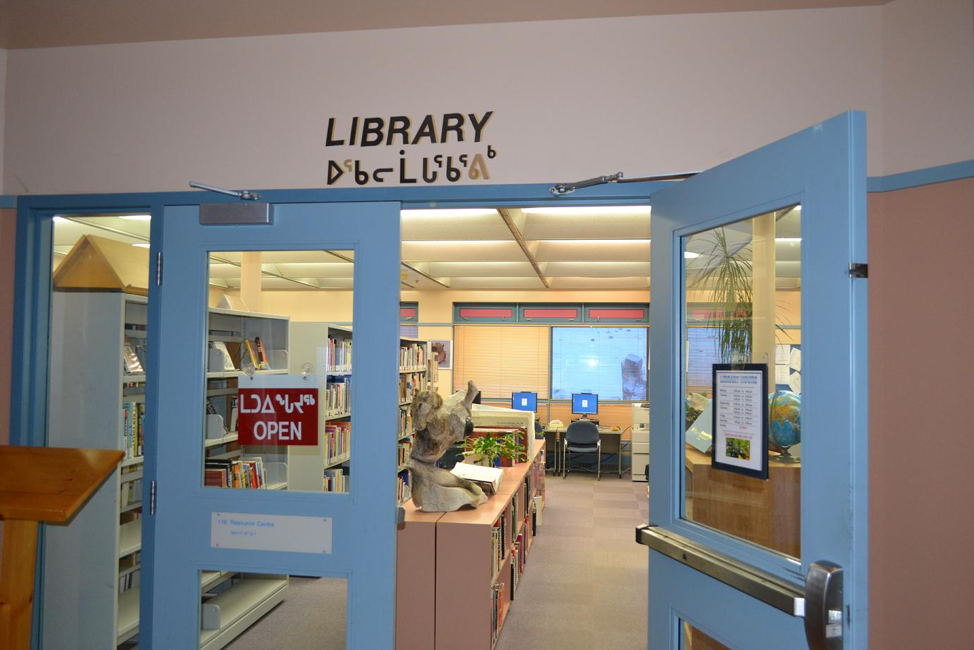
\includegraphics[width=.7\textwidth]{img/fig2.png}
\caption{Indigenous Language Signage}
\end{figure}

Library support of Indigenous Arctic language use can appear in
different types of libraries as well. The Maani Ulujuk Ilinniarvik
library in Rankin Inlet, Nunavut, for example serves as a library for
both high school students and community members who are Inuktitut
speakers. It carries books in both Inuktitut and Inuinnaqtun for their
use (Dumancic, 2011). And the Legislative Library in Nunavut
\enquote{needs to have staff with good written and oral Inuktitut and
English language capability to provide services} (Earle, 2008, p.~3).
Further law library support for Indigenous speakers can be seen as well
in the establishment of the Akitsiraq Law School in Nunavut (Ableson,
2006).

\hypertarget{language-learning}{%
\section{Language Learning}\label{language-learning}}

In addition to supporting Indigenous speakers, libraries can also
potentially support other language learners as well, as for example, in
supporting learning for those with no prior knowledge of the language
but with a desire to learn it.

This library support could take the form of supplying beginner learner
materials to these library users. For example, the Juneau Public Library
in Alaska (also a part of the North, even if outside Canada) recently
sponsored language learning workshops in its space for Tlingit, a
Indigenous Arctic language in Alaska.\footnote{{[}\url{https://www.alaskapublic.org/2017/07/06/free-tlingit-workbook-part-of-language-revitalization/}}
In addition to offering space and supplies (tables, chairs,
whiteboards), the library also made available online access to a free
Tlingit workbook (Barrett, 2017).\footnote{\url{http://www.sealaskaheritage.org/sites/default/files/BeginningTlingitWorkbook.pdf}}

Another language learning support that libraries can offer is making
materials in Indigenous Arctic languages accessible to those wishing to
learn these languages. Carol Rigby, for example, devised a
classification scheme in order to catalogue a series of Inuktitut
curriculum materials that can strongly support language learning (Rigby,
2007). In more recent work, Rigby has continued to promote the use of
Indigenous Arctic language into cataloguing standards even through
commercial vendors (Rigby, 2015).

Helping to celebrate academic achievement in the learning of a
Indigenous Arctic language is another example of libraries supporting
language education. At the University of Alaska Southeast in November
2017, for example, a student at the university was the first person to
ever earn a Tsimshian language credit in the United States, and her
celebration was held at the campus library (Dudzak, 2017). And the
learning about Indigenous Arctic languages and cultures can occur in the
other direction as well, as reported by a librarian who was hired to
work on an adult literacy project in Kugluktuk, Nunavut (Mulder, 2003).

\hypertarget{language-research}{%
\section{Language Research}\label{language-research}}

Another component of language education that libraries can support
beyond language use and language learning is language research. By
supporting and helping to develop research about Indigenous Arctic
languages, librarians can also serve an important role in Indigenous
Arctic language education. This could be done by becoming aware of
specialized polar research being done about the Arctic, and then by
sharing or making that information accessible to their library users.

Often this specialized research can be found through current conference
proceedings. One example of such a conference was the 2017 Ninth
International Conference on Arctic Social Sciences that took place in
Umea, Sweden .\footnote{\url{http://www.trippus.se/web/Presentation/web.aspx?evid=l+k2p0UcaP8eXy9TNfnXsQ==\&ecid=loNJV+HVzL0o7zbDGv/zsQ==\&ln=eng\&view=category\&template=desktoph}}
Another such conference is the upcoming 2018 Polar Libraries Colloquy
convened on the theme of \enquote{Developing Polar Networks: Ideas \&
Possibilities for the Future}.\footnote{\url{https://polarlibraries.org/27th-polar-libraries-colloquy/}}

Another example can be found in specialized web sites devoted to topics
in Arctic research. One such web site comes from a consortial group
called the University of the Arctic, which describes itself as a
\enquote{cooperative network of universities, colleges, research
institutes, and other organizations concerned with the education and
research in and about the North} .\footnote{\url{https://www.uarctic.org/about-uarctic/}}
This web site can provide a wide portal to the scholarship of the Arctic
for interested librarians. The Arctic Lingua thematic network, in
particular, serves as a very specialized clearinghouse for polar
research that focuses on Indigenous Arctic languages through language
documentation and language technologies studies.\footnote{\url{https://www.uarctic.org/organization/thematic-networks/arctic-lingua/}}

\hypertarget{language-and-cultural-preservation}{%
\section{Language and Cultural
Preservation}\label{language-and-cultural-preservation}}

Moving beyond the support of language research, library support through
cultural preservation work is another avenue that libraries can use to
support Indigenous Arctic language education. As with the other types of
library support above, this can also take many forms.

One such way is through resource sharing projects. Yvonne Earle
describes the creation of this type of a project by using the example of
creating and developing a catalogue of Indigenous wildlife resources in
Nunavut (Earle, 2003). While potentially not teaching use of an Arctic
language, this project still preserves cultural knowledge about life in
the Arctic for Inuit.

A similar example is that of a photographic web project, Project Naming,
which was described by David A. Smith in 2008. This project, in part,
brought together visual images from Nunavut as well as Micronesia, and
solicited Indigenous input from people of those regions to improve the
descriptions of the photographs. A project of this nature also helps
preserve the culture of Arctic people while also preserving Indigenous
names of individuals appearing in its contents (Smith, 2008).

Informing much of the present day preservation of both the language and
culture of the Inuit is a set of principles called the Inuit
Qaujimajatuqangit (IQ Principles) that deserves mention here as well.
This set of principles emerged from Inuit values and beliefs, and it
includes much content on languages of instruction that need to be
supported when developing curriculum guides in Nunavut. Shelby's
grandfather played a direct role in the production of this manual
describing these principles.\footnote{\url{https://www.gov.nu.ca/sites/default/files/files/Inuit\%20Qaujimajatuqangit\%20ENG.pdf}}

In terms of library applicability to language and cultural preservation,
the importance of applying the IQ principles to a library environment is
well described by Patricia Doucette, a non-Indigenous librarian who
served as the Manager of Library Services at Nunavut Arctic College from
1999 to 2003 (Doucette, 2003). In this article, she makes the
interesting point that,

\begin{quote}
\enquote{Seventy-seven per cent of the respondents identified
audiovisual materials as the resource to which they most wanted access.
I believe that this preference directly relates to the nature of Inuit
culture. As a medium for the provision of information, a video is much
more familiar than written materials to people who are accustomed to
being taught through oral traditions.} (Doucette, 2003, pp.~261--262).
\end{quote}

This comment is supported by research done in the field of adult
education as well that looks at the preferred use of incorporating
visual learning into classes of other Arctic peoples in Western Canada
(Robinson, 2009). It also emphasizes our initial opening comment at the
start of this article, that understanding the Arctic may often seem to
involve images in addition to words.

\hypertarget{language-publishing-opportunities}{%
\section{Language Publishing
Opportunities}\label{language-publishing-opportunities}}

Shifting back to written language support, opportunities to help with
the publishing of books in Indigenous Arctic languages is the last
category we identified in our document analysis as a way that libraries
can support language education.

An example of a book published in this way can be seen in a dictionary
of Inuktitut suffixes produced by the Arctic College Library of Nunavut
with the impressive title of ``\emph{UTKUHIKŠALINGMIUT UQAUHIITIGUT
UQAUHILIURUT. DICTIONARY OF UTKUHIKSALINGMIUT INUKTITUT POSTBASE
SUFFIXES}. This book was given a full book review in the journal
\emph{Arctic} that appeared in December of 2016 (Dorais, 2016,
pp.~435--436).

Another publishing support opportunity for libraries can occur through
spreading awareness or buying material for their collections that are
produced by Indigenous authors. One example of a library guide that has
collected information on Indigenous publishers is maintained by the
University of Toronto Libraries.\footnote{\url{https://guides.library.utoronto.ca/Aboriginalpublishers}}

There do exist Indigenous publishers of children's books who produce
work in Indigenous Arctic languages as well that could offer another
language education support mechanism for libraries. See, for example,
Inhabit Media's book on \emph{Inuit Innguiusingit: A Collection of Inuit
Choral Music}.\footnote{\url{https://inhabitmedia.com/2016/08/10/inuit-inngiusingit/}}

\hypertarget{future-opportunities-for-library-support}{%
\section{Future Opportunities for Library
Support}\label{future-opportunities-for-library-support}}

While performing the document analysis that resulted in the categories
and examples above, we also came across other documents and pieces of
information having to do with the Arctic that might lend themselves to
future library support possibilities.

These examples include fairly recent educational initiatives such as
Yukon College's introduction of \enquote{First Nations core competency
for all graduates} (Yukon College, 2015). As the only institution of
higher education in the Yukon Territory of Canada, this initiative is
worth paying attention to, because it could potentially include library
support in reaching this curricular goal. It could also potentially
involve library language material provision and services in addition.
Yukon College is also currently undergoing the process of transforming
from a college into a university, and it has proposed new degrees such
as a Bachelor of Arts in Indigenous Governance, which might have library
ramifications as well (Yukon Government, 2017).

A similar educational initiative is playing out at the University of
Prince Edward Island. In this case, the Faculty of Education at the
University is partnering with the Government of Nunavut to offer the
\enquote{first-ever graduate-level course taught in Inuktitut}
(University of Prince Edward Island, 2017). With a Indigenous Arctic
language serving as the language of instruction, library support could
also help strengthen the student experience, so this initiative bears
watching as well.

Both of these initiatives seemed poised to promote growing calls for
incorporating more Indigenous learning opportunities into higher
education circles in Canada in the coming years (Chiose, 2017). As a
counterpoint to these seemingly positive announcements, however, it must
also be noted that unhappy developments have occurred recently as well.
Peter Varga, in a newspaper article decrying the lack of a university in
the Arctic, stated that, \enquote{Nunavummiut and other peoples of the
Canadian Arctic have little chance of shaping the development of their
northern lands and culture without an Arctic-based university run by
peoples of the region, for peoples of the region} (Varga, 2017).

\hypertarget{need-for-further-research}{%
\section{Need for Further Research}\label{need-for-further-research}}

The need for future study of how libraries can best support Arctic
language education remains immense. Besides a more in-depth
consideration of the examples offered above, a deeper understanding of
the contexts that these examples come from and operate in would also go
far in strengthening future library support.

One key element to a deeper contextual understanding would be the
ability to hear more directly the voices of more Indigenous language
users in the Arctic as to what their library needs and desires are. The
importance of understanding Inuit knowledge when studying the Arctic
must be acknowledged. In addition, more voices of librarians working in
this region would be welcome as well.

One very rare example of hearing both voices at once, that of an
Indigenous speaker as well as of a practicing librarian in the Arctic,
can perhaps provide some direction for the future. In a paper presented
at the 19\textsuperscript{th} annual Polar Libraries Colloquy in
Copenhagen, Denmark, in 2002, one presentation entitled \enquote{A
Greenlandic Inuk librarian's point of view on the future of Inuit
libraries, language and literature} was offered by a librarian from the
National Public Library of Greenland (Jermiassen, 2002). In this paper,
she addresses library challenges such as orthography (spelling changes)
in the Indigenous language, the lack of funds needed to classify much
primary source material, and the unique cultural setting of Greenland as
factors to consider in library work in this region. Laying out such a
groundwork can help plot the future course of research concerning
libraries and the Arctic.

\hypertarget{conclusion}{%
\section{Conclusion}\label{conclusion}}

Libraries do have a role to play in supporting Indigenous Arctic
language education. This support can play out in a number of different
ways: by supporting Indigenous speakers and language learners through
library material collection and support, by designating the library as a
physical place in which to use and study these languages, by supporting
and making available research about the Arctic, by participating in
cultural and language preservation efforts, and by providing awareness
or direct support of publishing opportunities. In conclusion, supporting
Indigenous Arctic language education in and through libraries can open
the door to one small way of potentially expanding understandings of the
Arctic through the field of librarianship.

\hypertarget{references}{%
\section{\texorpdfstring{\textbf{References}}{References}}\label{references}}

Ableson, S. (2006). Bringing legal education to the Canadian Arctic: The
development of the Akitsiraq Law School and the challenges for providing
library services to a non-traditional law school. \emph{International
Journal of Legal Education, 34} (1): 1--30. Available online at
\url{https://scholarship.law.cornell.edu/ijli/vol34/iss1/4}.

Arcadia, S. (2011). \enquote{Arctic research: Environment, health, and
culture of the circumpolar north.} \emph{College \& Research Libraries
News, 72} (2): 104--107. Available online at
\url{https://doi.org/10.5860/crln.72.2.8513}.

Barrett, C. (July 5, 2017). \emph{Free Tlingit Workbook Part of Language
Revitalization}. KT-00 Juneau. Available online at
\url{https://www.alaskapublic.org/2017/07/06/free-tlingit-workbook-part-of-language-revitalization/}.

Campbell, M. (March 3, 2017). \enquote{Get ready for a Canadian Arctic
research boom.} \emph{Macleans}. Available online at
\url{http://www.macleans.ca/society/science/get-ready-for-a-canadian-arctic-research-boom/}.

Charron, A., Plouffe, J., \& Roussel, S. (March 2012). \enquote{The
Russian Arctic hegemon: Foreign policy implications for Canada.}
\emph{Canadian Foreign Policy, 18} (1), 38--50. Available online at
\url{https://doi.org/10.1080/11926422.2012.674384}.

Chiose, S. (2017). A curriculum of their own. \emph{Globe and Mail},
January 2, 2018. Available online at
\url{https://www.theglobeandmail.com/news/national/as-number-of-indigenous-grads-grows-so-do-calls-for-funding-and-curriculum-changes/article37477177/}.

Coad, B. W. \& Reist, D. D. (2018). \emph{Marine Fishes of Arctic
Canada}. Toronto: Canadian Museum of Nature.

Comrie, B. (September 1991). Review of \emph{Arctic Languages: An
Awakening} by Dirmid R. F. Collis. \emph{Language, 67} (3): 624--627.
Available online at \url{https://doi.org/10.1353/lan.1991.0033}.

Dorais, L. (1995). Language, culture and identity: Some Inuit examples.
\emph{Canadian Journal of Native Studies, 15} (no issue): 293--308.

Dorais, L. (December 2016). UTKUHIKŠALINGMIUT UQAUHIITIGUT UQAUHILIURUT.
DICTIONARY OF UTKUHIKSALINGMIUT INUKTITUT POSTBASE SUFFIXES.
\emph{Arctic, 69} (4), 435--436.

Doucette, P. (2003). \enquote{Incorporating Inuit Qaujimajatuqangit into
library service and programs -- or vice versa?} \emph{Feliciter, 49}
(5): 260--262.

Dudzak, M. (December 6, 2017). \enquote{UAS student first in U.S. to
receive Tsimshian language credential.} KRBD radio news, Ketchikan,
Alaska. Available online at
\url{https://www.ktoo.org/2017/12/06/uas-student-first-u-s-receive-tsimshian-language-credential/}.

Dumancic, M. (Spring 2011). \enquote{A page from Canada's north.}
\emph{Access, 17} (2): 34--35.

Earle, Y. (2003). \enquote{Making resources go farther: A
resource-sharing project in Nunavut.} Feliciter, 49 (3): 150--153.

Earle, Y. (2008). Ikajarutit: Delivering legislative library services in
aboriginal language environment (Nunavut, Canada). \emph{World Library
and Information Conference: 74\textsuperscript{th} IFLA General
Conference and Council}. Quebec, Canada. Available online at
\url{https://archive.ifla.org/IV/ifla74/papers/103-Earle-en.pdf}.

Firth, M. (Spring 2017). Alone across the Arctic. \emph{Surgite: A Brock
Community Magazine, 9} (1), 12--13.

Gettler, B. (December 2017). Historical research at the Truth and
Reconciliation Commission of Canada." \emph{Canadian Historical Review,
98} (4), 641--674. Available online at
\url{https://doi.org/10.3138/chr.98.4.641}.

\emph{Global Literature in Libraries Initiative} (2017). Available
online at \url{https://glli-us.org/about/}.

Gonzalez, R. G. (2017). \enquote{Internationalization at a German
university: The purpose and paradoxes of English language.} \emph{The
International Education Journal: Comparative Perspectives, 16} (2),
49--62. Available online at
\url{https://openjournals.library.usyd.edu.au/index.php/IEJ/article/view/10312}.

Griffiths, F.; Huebert, R.; \& Lackenbauer, P. W. (2011). \emph{Canada
and the Changing Arctic: Sovereignty, Security, and Stewardship}.
Waterloo, ON: Wilfred Laurier Press.

Hall, P. A. (1992). \enquote{Peanuts: A note on intercultural
communication.} \emph{The Journal of Academic Librarianship, 18} (3),
211--213.

Hoag, H. (September 19, 2017). Canada's new Arctic research station
readies for its grand opening. \emph{University Affairs}. News blog.
Available online at
\url{https://www.universityaffairs.ca/news/news-article/canadas-new-arctic-research-station-readies-grand-opening/}.

Jermiassen, E. (2002). \enquote{A Greenlandic Inuk librarian's point of
view on the future of Inuit libraries, language and literature.}
\emph{19\textsuperscript{th} annual Polar Libraries Colloquy}.
Copenhagen, Denmark. Available online at
\url{http://arcticcentre.ulapland.fi/polarweb/plc/pdf/plc02_full.pdf}.

Johnston, P. \& Tester, F. (2014). \enquote{Breaking the colonial role:
Changing social work practices in Nunavut.} \emph{Canadian Journal of
Native Studies, 34} (1), 111--127.

MacDonald, P. (December 27, 2017). Mi'kmaq leader seeks official
language designation in Nova Scotia. \emph{CBC News}. Available online
at
\url{http://www.cbc.ca/news/canada/nova-scotia/mi-kmaq-language-leroy-denny-eskasoni-cbu-1.4462562}.

Mulder, M. (January 20, 2003). \enquote{In an Arctic library.}
\emph{Macleans, 116} (3), 43.

Pucci, M. (June 19, 2017). \enquote{A core part of our identity}:
Indigenous language law targeted for 2018. \emph{CBC News}. Available
online at
\url{http://www.cbc.ca/news/canada/north/indigenous-language-inuktut-natan-obed-1.4168017}.

Rathwell, K. J. \& Armitage, D. (2016). \enquote{Art and artistic
processes bridge knowledge systems about social-ecological change: An
empirical examination with Inuit artists from Nunavut, Canada.}
\emph{Ecology \& Society, 21} (2), 310--323. Available online at
\url{https://doi.org/10.5751/ES-08369-210221}.

Rigby, C. (2007). \enquote{Nunavut curriculum materials relocated and
reorganized.} \emph{Partnership: The Canadian Journal of Library and
Information Practice and Research, 2} (1), 6.

Rigby, C. (2015). \enquote{Nunavut libraries online establish Inuit
language bibliographic cataloging standards: Promoting indigenous
language using a commercial ILS.} \emph{Cataloging \& Classification
Quarterly, 53} (5): 615--639. Available online at
\url{https://doi.org/10.1080/01639374.2015.1008165}.

Robinson, S. (2009). \enquote{Literacy lives here: Using video and
dialogue to promote and celebrate adult and literacy education in the
Canadian western Arctic.} \emph{New Directions for Adult \& Continuing
Education, 124}, 15--23. Available online at
\url{https://doi.org/10.1002/ace.349}.

Smith, D. A. (2008). \enquote{From Nunavut to Micronesia: Feedback and
description, visual repatriation and online photographs of indigenous
peoples.} \emph{Partnership: The Canadian Journal of Library and
Information Practice and Research, 3} (1), 1--19. Available online at
\url{https://doi.org/10.21083/partnership.v3i1.330}.

Sraku-Lartey, M.; Britwum Acquah, S.; Samar, S. B.; \& Djagbletey, G. D.
(2017). \enquote{Digitization of indigenous knowledge on forest foods
and medicines.} \emph{IFLA Journal, 43} (2), 187--197. Available online
at \url{https://doi.org/10.1177/0340035216681326}.

University of Prince Edward Island (2017). UPEI, Government of Nunavut
to offer first-ever graduate-level course taught in Inuktitut.
\emph{University of Prince Edward Island News}, July 21, 2017. Available
online at
\url{http://www.upei.ca/communications/news/2017/07/upei-government-nunavut-offer-first-ever-graduate-level-course-taught-inuktitut}.

\emph{Using Libraries to Support National Literacy Efforts} (2016). UIL
(UNESCO Institute for Lifelong Learning) Policy Brief 6. Available
online at \url{http://unesdoc.unesco.org/images/0024/002467/246778e.pdf}

Vargas, P. (2017). Politics, power, money real culprits behind nixing
Arctic University. \emph{Nunatsiaq Online}, March 27, 2017. Available
online at
\url{http://www.nunatsiaqonline.ca/stories/article/65674politics_power_money_real_culprits_behind_nixing_arctic_university_sau/}.

Yukon College (2015). Yukon College introduces First Nations core
competency for all graduates. \emph{Yukon College News}, October 6,
2015. Available online at
\url{https://www.yukoncollege.yk.ca/news/P108}.

Yukon Government (2017). Yukon College recognized as ready to offer
undergraduate degree programs. \emph{Yukon Government News Release},
December 14, 2017. Available online at
\url{http://www.gov.yk.ca/news/17-268.html}.

Zellen, B. S. (2013). \emph{The Fast-Changing Arctic: Rethinking Arctic
Security for a Warmer World}. Calgary, AB: University of Calgary Press.

Zeller, S. \& Ries, C. J. (April 2014). Wild men in and out of science:
Finding a place in the disciplinary borderlands of Arctic Canada and
Greenland. \emph{Journal of Historical Geography, 44} 31--43. Available
online at \url{https://doi.org/10.1016/j.jhg.2013.12.002}.

%autor
\begin{center}\rule{0.5\linewidth}{\linethickness}\end{center}

\textbf{Karen Bordonaro}, is a liaison librarian at Brock University,
Ontario, Canada. She studies internationalization in academic libraries,
as well as linguistic uses of libraries by non-Indigenous speakers of
English in various settings within and outside the United States and
Canada.

\textbf{Shelby Angalik}, Inuk from Nunavut, is a current Brock
University undergraduate student majoring in English who is considering
the profession of librarianship as a possible future career.

\end{document}
